\documentclass{article}
\usepackage[utf8]{inputenc}
\usepackage{hyperref}
\usepackage[letterpaper, portrait, margin=1in]{geometry}
\usepackage{enumitem}
\usepackage{amsmath}
\usepackage{booktabs}
\usepackage{graphicx}

\usepackage{hyperref}
\hypersetup{
colorlinks=true,
    linkcolor=black,
    filecolor=black,      
    urlcolor=blue,
    citecolor=black,
}
\usepackage{natbib}

\usepackage{titlesec}

\title{Homework 4}
\author{Roshani Bulkunde}
\date{February 2023}

\begin{document}

\maketitle

\section{Python}

\subsection{Question 1}

\begin{figure}[ht]
    \centering
    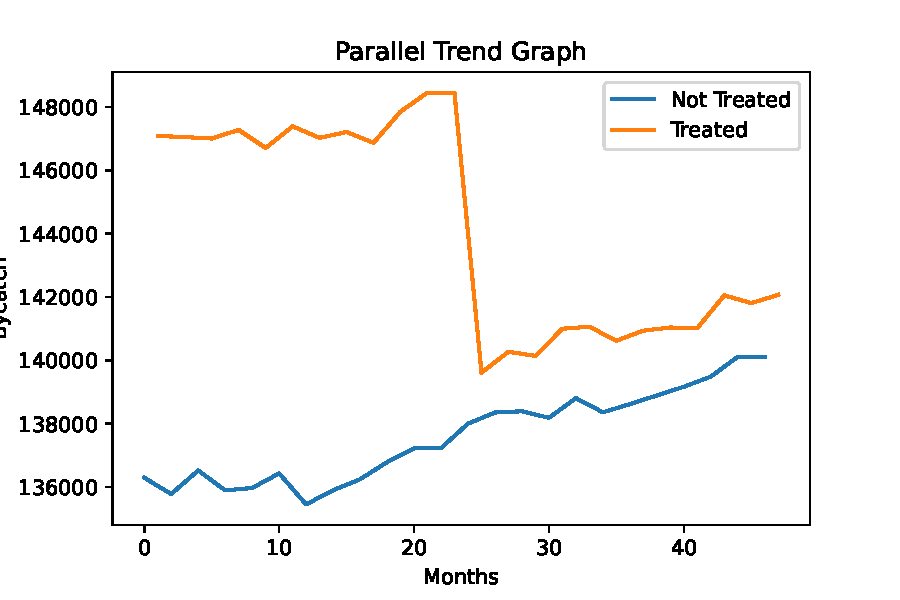
\includegraphics[scale = 0.7]{paralleltrend.pdf}
    \caption{Parallel trends of bycatch}
    \label{fig:paralleltrend}
\end{figure}

From figure \ref{fig:paralleltrend}, I can say there are parallel trends before the treatment. 

\subsection{Question 2}
The DID estimate is -68374.51. The intuition of this estimate is that bycatch is reduced by -68374.51 in the firms that received the best practices to reduce bycatch compared to the firms that did not receive the information.

\subsection{Question 3 (a)}
\begin{table}[ht]
    \centering
    \begin{tabular}{lr}
\toprule
{} &          0 \\
\midrule
T=2017 intercept &    -773.22 \\
                 &   23970.28 \\
Treatment        &   11202.04 \\
                 &   23065.41 \\
Treatment*Post   &   -9591.35 \\
                 &   32619.42 \\
Constant         &  138001.81 \\
                 &   16949.55 \\
Observations     &     100.00 \\
\bottomrule
\end{tabular}

    \caption{Question 3a without clustered standard errors }
    \label{tab:DID3a_python}
\end{table}

\begin{table}[ht]
    \centering
    \begin{tabular}{lr}
\toprule
{} &          0 \\
\midrule
T=2017 intercept &    -773.22 \\
                 &     598.69 \\
Treatment        &   11202.04 \\
                 &   23502.90 \\
Treatment*Post   &   -9591.35 \\
                 &    3231.79 \\
Constant         &  138001.81 \\
                 &   18657.80 \\
Observations     &     100.00 \\
\bottomrule
\end{tabular}

    \caption{Question 3a with clustered standard errors }
    \label{tab:DID3a_clusterstd_python}
\end{table}

Table \ref{tab:DID3a_clusterstd_python} reports the coefficient estimates and clustered-standard errors in the bracket. The sample includes the observations in December 2017 and January
2018 only. 

\newpage

\subsection{Question 3 (b)}
\begin{table}[ht]
    \centering
    \begin{tabular}{ll}
\toprule
{} &          0 \\
\midrule
Firm           &     876.02 \\
               &   (153.42) \\
Month          &     6589.7 \\
               &   (355.15) \\
Treatment      &   83180.73 \\
               &  (5835.91) \\
Treatment*Post &  -85470.13 \\
               &  (8401.58) \\
Observations   &     1200.0 \\
\bottomrule
\end{tabular}

    \caption{Question 3b without clustered standard errors }
    \label{tab:DID3b_python}
\end{table}

\begin{table}[ht]
    \centering
    \begin{tabular}{ll}
\toprule
{} &           0 \\
\midrule
Firm           &      876.02 \\
               &    (679.56) \\
Month          &      6589.7 \\
               &   (1182.82) \\
Treatment      &    83180.73 \\
               &  (20049.39) \\
Treatment*Post &   -85470.13 \\
               &  (14341.32) \\
Observations   &      1200.0 \\
\bottomrule
\end{tabular}

    \caption{Question 3b with clustered standard errors }
    \label{tab:DID3b_clusterstd_python}
\end{table}

Table \ref{tab:DID3b_clusterstd_python} reports the coefficients which estimate the treatment effect of the program on bycatch using a regression-based difference-in-differences estimator using the regression. Using this estimation, the coefficient can be interpreted as bycatch reduced by -85470.13 in the firms that received the information about best practices to reduce bycatch compared to the firms that did not receive the information. The reduction in the bycatch in part b is smaller than the part a.

\newpage

\subsection{Question 3 (c)}
\begin{table}[ht]
    \centering
    \begin{tabular}{lr}
\toprule
{} &         0 \\
\midrule
Firm           &    -61.68 \\
               &     12.81 \\
Month          &    124.92 \\
               &     33.57 \\
Treatment      &   1292.98 \\
               &    507.51 \\
Treatment*Post & -10074.05 \\
               &    700.66 \\
Firmsize       &  -1125.76 \\
               &   1088.83 \\
Shrimp         &      1.04 \\
               &      0.02 \\
Salmon         &      0.55 \\
               &      0.07 \\
Observations   &   1200.00 \\
\bottomrule
\end{tabular}

    \caption{Question 3c without clustered standard errors }
    \label{tab:DID3c_python}
\end{table}

\begin{table}[ht]
    \centering
    \begin{tabular}{ll}
\toprule
{} &          0 \\
\midrule
Firm           &     -61.68 \\
               &    (26.65) \\
Month          &     124.92 \\
               &    (62.46) \\
Treatment      &    1292.98 \\
               &   (663.72) \\
Treatment*Post &  -10074.05 \\
               &  (3270.82) \\
Firmsize       &   -1125.76 \\
               &  (3196.23) \\
Shrimp         &       1.04 \\
               &     (0.05) \\
Salmon         &       0.55 \\
               &     (0.19) \\
Observations   &     1200.0 \\
\bottomrule
\end{tabular}

    \caption{Question 3c with clustered standard errors }
    \label{tab:DID3c_clusterstd_python}
\end{table}

Table \ref{tab:DID3c_clusterstd_python} reports the coefficients and clustered-standard errors, estimating the difference-in-differences regression with added controls. Using this estimation, the coefficient can be interpreted as bycatch reduced by  -10074.05 in the firms that received the information about best practices to reduce bycatch compared to the firms that did not receive the information. The reduction in the bycatch in part c is smaller than in part a and part b.

\newpage


\subsection{Question 3 (d)}
\begin{table}[ht]
    \centering
    \begin{tabular}{llll}
\toprule
{} &        (3a) &        (3b) &       (3c) \\
0              &             &             &            \\
\midrule
Treatment      &    11202.04 &    83180.73 &    1292.98 \\
               &  (23502.90) &  (20049.39) &   (663.72) \\
Treatment*Post &    -9591.35 &   -85470.13 &  -10074.05 \\
               &   (3231.79) &  (14341.32) &  (3270.82) \\
Firmsize       &             &             &   -1125.76 \\
               &             &             &  (3196.23) \\
Shrimp         &             &             &       1.04 \\
               &             &             &     (0.05) \\
Salmon         &             &             &       0.55 \\
               &             &             &     (0.19) \\
Observations   &       100.0 &      1200.0 &     1200.0 \\
\bottomrule
\end{tabular}

    \caption{Question 3d with clustered standard errors }
    \label{tab:output3d_python}
\end{table}

Table \ref{tab:output3d_python} reports the results from (a), (b), and (c) in a table with standard errors calculated using clustered standard errors at the firm level. The coefficient of the interaction term treatment*post is our coefficient of interest. In part a (column 3a), the coefficient can be interpreted as the bycatch reduced by (138001.81 - 9591.35 =128,410) in the firms which received the program as compared to the programs that did not receive the program. In part 3b, the bycatch reduced by -85470.13 as the effect of the program. In part 3b, we add controls to estimation 3b, and the bycatch reduced to -10074.05 as the effect of the program.

\newpage

\section{STATA}

\subsection{Question 1 (a)}
\begin{table}[ht]
    \centering
    \begin{tabular}{lc} \hline
 & (1) \\
VARIABLES & Bycatch \\ \hline
 &  \\
Firm ID & -109.5** \\
 & (41.87) \\
Month & -2.274 \\
 & (29.29) \\
Treatment & -8,674*** \\
 & (2,742) \\
Firmsize & -966.0 \\
 & (3,222) \\
Shrimp (Pounds) & 1.044*** \\
 & (0.0500) \\
Salmon (Pounds) & 0.529** \\
 & (0.200) \\
Constant & 4,777** \\
 & (1,998) \\
 &  \\
Observations & 1,200 \\
 R-squared & 0.992 \\ \hline
\multicolumn{2}{c}{ Robust standard errors in parentheses} \\
\multicolumn{2}{c}{ *** p$<$0.01, ** p$<$0.05, * p$<$0.1} \\
\end{tabular}

    \caption{Question 1a with clustered standard errors }
    \label{tab:q1a_cluster_stata}
\end{table}

\subsection{Question 1 (b)}
\begin{table}[ht]
    \centering
    \begin{tabular}{lc} \hline
 & (1) \\
VARIABLES & Demeaned Bycatch \\ \hline
 &  \\
Demeaned post*treated & -8,149*** \\
 & (2,489) \\
Demeaned Firmsize = o, & - \\
 &  \\
Demeaned Shrimp (Pounds) & 1.537*** \\
 & (0.179) \\
Demeaned Salmon (Pounds) & -0.428 \\
 & (0.598) \\
Constant & -0.000241 \\
 & (0.000902) \\
 &  \\
Observations & 1,200 \\
 R-squared & 0.426 \\ \hline
\multicolumn{2}{c}{ Robust standard errors in parentheses} \\
\multicolumn{2}{c}{ *** p$<$0.01, ** p$<$0.05, * p$<$0.1} \\
\end{tabular}

    \caption{Question 1b with clustered standard errors }
    \label{tab:q1b_cluster_stata}
\end{table}

\newpage

\subsection{Question 1 (c)}
\begin{table}[ht]
    \centering
    \begin{tabular}{lcc} \hline
 & (1) & (2) \\
VARIABLES & Bycatch & Demeaned Bycatch \\ \hline
 &  &  \\
post*treated & -8,320*** &  \\
 & (2,650) &  \\
Firmsize = o, & - &  \\
 &  &  \\
Shrimp (Pounds) & 1.531*** &  \\
 & (0.172) &  \\
Salmon (Pounds) & -0.610 &  \\
 & (1.088) &  \\
Demeaned post*treated &  & -8,149*** \\
 &  & (2,489) \\
Demeaned Firmsize = o, &  & - \\
 &  &  \\
Demeaned Shrimp (Pounds) &  & 1.537*** \\
 &  & (0.179) \\
Demeaned Salmon (Pounds) &  & -0.428 \\
 &  & (0.598) \\
Constant & 186,390 & -0.000241 \\
 & (238,156) & (0.000902) \\
 &  &  \\
Observations & 1,200 & 1,200 \\
 R-squared & 0.996 & 0.426 \\ \hline
\multicolumn{3}{c}{ Robust standard errors in parentheses} \\
\multicolumn{3}{c}{ *** p$<$0.01, ** p$<$0.05, * p$<$0.1} \\
\end{tabular}

    \caption{Question 1 c with clustered standard errors }
    \label{tab:q1c_stata}
\end{table}
Column (1) of table \ref{tab:q1c_stata} are the estimates from part 1(a) and column (2) are the estimates from part 1(b). The coefficient of the interaction term treatment*post is our coefficient of interest. In part a (column 1), the coefficient can be interpreted as the bycatch is reduced by 8320 in the firms which received the program as compared to the programs that did not receive the program. Using the within transformation in part b we are controlling for fixed effects. In part b, the bycatch is reduced by 8149 where received the information as compared to the firms that did not receive the information.
\end{document}